\documentclass[GAP.tex]{subfiles}
\begin{document}

\chapter{Tema 1}
\begin{dem}[Proposición 2] Sean M una superficie una superficie regular y $f:M\to\R$ una aplicación continua, $p\in M$ y $(U,\X)$ una superficie simple tal que $p \in \X(U)$ y satisface las condiciones de la Definición 1. Sea otra superficie simple $(V,\Y)$ en las condiciones anteriores. Como $(U,\X)$ y $(V,\Y)$ son superficies simples de una misma superficie regular, deben ser compatibles en la intersección. Es decir, podemos considerar la aplicación diferenciable $\X^{-1}\circ \Y \func{\Y^{-1}(W)}{X^{-1}(W)}$, donde $W=\X(U)\cap\X(V)$. Consideramos:
\[
f\circ \Y = (f \circ \X)\circ (\X^{-1}\circ \Y)
\]
Como todas las aplicaciones son diferenciables, deducimos que $f\circ \Y$ también lo es en $p''=\Y^{-1}(p)$.

\QED
\end{dem}
\begin{dem}[Proposición 3] Sea $f\func{\R^3}{\R}$ una aplicación diferenciable. Sea M una superficie regular en $\R^3$. Tenemos que $f$ es continua en $\R^3$, de donde se deduce que $f|_M$ es continua. En efecto, sea $I\subset \R$ abierto, $f^{-1}|_M(I)\cap M = f^{-1}(I)\cap M  \subset M$ abierto relativo, por lo que es continua. Sea $p\in M$. Veamos que $f|_M$ es diferenciable en $p$. Sea $(U,\X)$ una s.s. de M en $p$. Entones $f|_M \circ \X = f \circ \X$, puesto que $X(U)\subset M$. Por tanto, $f\circ \X$ es diferenciable en $U$ y $p'\in U \subset \R^2$ abierto.\QED
\end{dem}
\begin{dem}[Proposición 9] 
Sea $p\in M$, $(U_1,\X_1)$ tal que $p\in\X_1(U_1)$ y $(V_1,\Y_1)$ tal que $f(p)\in\Y(V_1)$ satisfaciendo las condiciones de la definición 7. Sean  $(U_2,\X_2)$ y $(V_2,\Y_2)$ cumpliendo las mismas condiciones. Como las cartas son compatibles en sus respectivas superficies, podemos considerar las aplicaciones diferenciables $\Y_2^{-1}\circ \Y_1$ y $\X_1^{-1}\circ \X_2$. Por tanto, $$\Y_2^{-1}\circ f\circ \X_2=(\Y_2^{-1}\circ \Y_1)\circ (\Y_1^{-1}\circ f\circ\X)\circ(\X_1^{-1}\circ \X_2).$$
Así pues, $\Y_2^{-1}\circ f\circ \X_2$ es diferenciable en $p''=\X_2^{-1}(p)$ por ser composición de diferenciables.\QED
\end{dem}
\begin{dem}[Teorema 10] Sea $f\func{\R^3}{\R^3}$ una aplicación diferenciable, entonces, en particular, es continua. Sean M y N dos superficies regulares en $\R^3$ con $f(M)=N$. Veamos que $f|_M\func{M}{N}$ es continua. Sea $H\subset N$ abierto, $\exists J\subset \R^3$ abierto tal que $G=J\cap N$. Entonces $f|_M^{-1}(H) = f^{-1}(H)\cap M = f^{-1}(J\cap N)\cap M=f^{-1}(J)\cap f^{-1}(N)\cap M = f^{-1}(J)\cap M$ abierto relativo en M, puesto que $F^{-1}(J)\subset \R^3$ es abierto. Luego, $f|_M$ es continua.\QED

Sea $p\in M$. Veamos que $f|_M\func{M}{N}$ es diferenciable en $p$. Sea $(U,\X)$ una s.s. de M en $p\in\X(U)$ y $(V,\Y)$ un s.s. en N con $f(p)\in\Y(V)$. Consideramos la composición en $\Y^{-1}\circ f \circ \X$, que tiene sentido en $\X^{-1}(W)$, donde $W = f^{-1}(\Y(V))\cap \X(U)$. Además, se tiene que $\Y^{-1}\circ f \circ \X = \Y^{-1}\circ f|_M \circ \X$ en $\X^{-1}(W)$ y es diferenciable por ser composición de funciones diferenciable en $p'=\X^{-1}(p)$. Por tanto $f|_M$ es diferenciable.\QED
\end{dem}

\begin{dem}[Teorema 17]
Sean $M$ y $N$ dos superficies regulares y sea $f:M\to N$ una aplicación diferenciable. Sea $p\in M$ y $\vec{v}\in T_p(M)$. Sean $(U,\X)$ y $(V,\Y)$ dos superficies simples en $M$ y $N$ respectivamente, con $p\in\X(U)$ y $f(p)\in\Y(V)$. Sea $\gamma:(-\varepsilon,\varepsilon)\to M$ una curva diferenciale en $M$ con $\gamma(0)=p$ y $\gamma'(0)=\vec{v}$. Podemos suponer WLOG que $\gamma(t)\in\X(U)\ \forall t\in(-\varepsilon,\varepsilon)$ y que $f\circ\gamma(t)\in\Y(V)\ \forall t\in(-\varepsilon,\varepsilon)$.  

Como $p\in\X(U)\Rightarrow p=\X(u_0^1,u_0^2)$, donde $u^1,u^2$ son los parámetros de la superficie simple $(U,\X)$. Como $\gamma$ es una curva diferenciable en $M$ y $\gamma(t)\in\X(U)\ \forall t\in(-\varepsilon,\varepsilon)$, entonces existen aplicaciones $u^1(t),u^2(t)$ tales que $\gamma(t)=\X(u^1(t),u^2(t))\ \forall t\in(-\varepsilon,\varepsilon)$. En particular, $p=\gamma(0)=\X(u^1(0),u^2(0))$, luego por la inyectividad de $\X$ deducimos que $u^1_0=u^1(0)$ y $u^2_0=u^2(0)$.  

Por otro lado $\vec{v}\in T_p(M)$ y $\{\X_1(u^1_0,u^2_0),\X_2(u^1_0, u^2_0)\}$ es una base de ese espacio, luego existen $\lambda^1,\lambda^2$ tales que 
$$\vec{v}=\lambda^1\X_1(u^1_0,u^2_0)+\lambda^2\X_2(u^1_0,u^2_0),$$
donde $\X_i(u^1_0,u^2_0)=\frac{\partial\X}{\partial u^i}|_{(u^1_0,u^2_0)}$. Tenemos $\vec{v}=\gamma'(0)$ y $\gamma(t)=\X(u^1(t),u^2(t))$, así que derivamos.
$$\vec{v}=\frac{\partial\X}{\partial u^1}|_{(u^1(0),u^2(0))}\frac{du^1}{dt}|_{t=0}+\frac{\partial\X}{\partial u^2}|_{(u^1(0),u^2(0))}\frac{du^2}{dt}|_{t=0}$$
Por tanto, como vimos antes que $u^1_0=u^1(0)$ y $u^2_0=u^2(0)$, $\lambda^i= \frac{du^i}{dt}|_{t=0}$. 

Ahora, $f(p)=f(\gamma(0))=f(\X(u^1_0,u^2_0)$ y $f(p)\in\Y(V)\Rightarrow\exists v^1_0, v^2_0\mid f(p)=\Y(v^1_0,v^2_0)$. Entonces $f\circ\gamma$ es una curva diferenciable en $N$ y $(f\circ\gamma)(t)\in\Y(V)\ \forall t\in(-\varepsilon,\varepsilon)$. Luego exsten aplicaciones $v^1(t),v^2(t)$ tales que $(f\circ\gamma)(t)=\Y(v^1(t),v^2(t))\ \forall t\in(-\varepsilon,\varepsilon)$. En particular, $(f\circ\gamma)(0)=f(p)=\Y(v^1_0,v^2_0)$, por lo que $v^1(0)=v^1_0$ y $v^2(0)=v^2_0$. Entonces, aplicando la regla de la cadena y sustituyendo $t=0$
$$f_{*p}\vec{v}=(f\circ\gamma)'(0)=\sum_{i=1}^2\frac{\partial\Y}{\partial v^i}|_{(v^1(0),v^2(0))}\frac{dv^i}{dt}|_{t=0}=\sum_{i=1}^2\Y_i(v^1_0,v^2_0)\frac{dv^i}{dt}|_{t=0}.$$
Por tanto, $f_{*p}\vec{v}\in T_{f(p)}(N)$ y $\{\Y_1(v^1_0,v^2_0),\Y_2(v^1_0,v^2_0)\}$ es una base de dicho espacio. Por ello existen $\mu^1,\mu^2$ tales que $$f_{*p}\vec{v}=\mu^1\Y_1(v^1_0,v^2_0)+\mu^2\Y_2(v^1_0,v^2_0).$$
Por lo anterior, sabemos que de hecho $\mu^1=\frac{dv^1}{dt}|_{t=0}$ y $\mu^2=\frac{dv^2}{dt}|_{t=0}$.

Como $f$ es diferenciable en $p$, la aplicación $\Y^{-1}\circ f\circ\X$ es diferenciable en un entorno abierto $\overline{U}$ de $p'=(u^1_0,u^2_0)$. Dado $(u^1,u^2)\in\overline{U}$, $\Y^{-1}\circ f\circ\X(u^1,u^2)=(v^1,v^2)=(v^1(u^1,u^2),v^2(u^1,u^2))$, por lo que

$$J_{p'}(\Y^{-1}\circ f\circ\X)=\begin{pmatrix}
\frac{\partial v^1}{\partial u^1} & \frac{\partial v^1}{\partial u^2}\\
\frac{\partial v^2}{\partial u^1} & \frac{\partial v^2}{\partial u^2}
\end{pmatrix}$$

Teniendo en cuenta las expresiones de $\lambda^i$ y $\mu^i$ podemos sustituir y encontrar
$$\mu^i=\frac{fv^i}{dt}|_{t=0}=\sum_{j=1}^2\frac{\partial v^i}{\partial v^j}|_{p'}\frac{du^j}{dt}|_{t=0}=\sum_{j=1}^2\frac{\partial v^i}{\partial u^j}|_{p'}\lambda^j$$
En conclusión, $f_{*p}$ es una aplicación lineal entre $T_p(M)$ y $T_{f(p)}(N)$, y la matriz de dicha aplicación respecto de las bases $\{\X_1(u^1_0,u^2_0),\X_2(u^1_0, u^2_0)\}$ y $\{\Y_1(v^1_0,v^2_0),\Y_2(v^1_0,v^2_0)\}$ es $J_{p'}(\Y^{-1}\circ f\circ\X)$. Además, la expresión para $f_{*p}\vec{v}$ es independiente de la curva diferenciable tomada. Con esto hemos demostrado la primera parte del teorema.

Para la segunda parte basta recordar que si la matriz de la aplicación lineal es regular, entonces la aplicación es biyectiva (por tanto isomorfismo). \QED

\end{dem}

\begin{ej}
Aplicación antipodal en $S^2$, es decir $f:S^2\to S^2$ definida por $f(x,y,z)=(-x,-y,-z)$. Ya vimos que $f$ es diferenciable. Sea $p\in S^2$ un punto fijado. Veamos cómo se define $f_{*p}$. Supongamos que $p$ está en el hemisferio norte de la esfera. Consideramos las superficies simples en $S^2$ siguientes:
$$\X:U\subseteq\R^2\to\R^3\mid \X(u^1,u^2)=(u^1,u^2,\sqrt{1-(u^1)^2+(u^2)^2})\quad\quad \Y:U\subseteq\R^2\to\R^3\mid \Y(u^1,u^2)=(u^1,u^2,-\sqrt{1-(u^1)^2+(u^2)^2}$$
Los abiertos serían $U=V=\{(x,y)\in\R^2\mid x^2+y^1<1\}$. Como ejercicio probar que efectivamente son superficies simples. Nos quedaría sin cubrir el ecuador.

Tomamos $(u^1,u^2)\in U$. Entonces $$\Y^{-1}\circ f\circ \X(u^1,u^2)=\Y^{-1}\circ f(u^1,u^2,\sqrt{1-(u^1)^2+(u^2)^2})=\Y^{-1}(-u^1,-u^2,\sqrt{1-(u^1)^2+(u^2)^2})=(-u^1,-u^2).$$
Por tanto $\Y^{-1}\circ f\circ \X:U\to V$ tal que $(u^1,u^2)\mapsto (-u^1,-u^2)=(v^1,v^2)$, por lo que su matriz jacobiana sería
$J_{p'}(\Y^{-1}\circ f\circ \X)=\begin{pmatrix}
\frac{\partial v^1}{u^1}	& \frac{\partial v^1}{u^2}\\
\frac{\partial v^2}{u^1}	& \frac{\partial v^1}{u^2}
\end{pmatrix}=\begin{pmatrix}
-1	& 0\\
0	& -1
\end{pmatrix}=-Id,$ con $p'=\X^{-1}(p)$. Por tanto $f_{*p}:T_p(S^2)\to T_{-p}(S^2)$ está definida como $\vec{v}\mapsto -\vec{v}$.
\end{ej}

Cada una de las definiciones de isometría son para sustituir la parte ``$f_{*p}$ es isometría''
\begin{defi}[Alternativa para isometría]
Si $f_{*p}$ es isometría $\forall p\in M$, por definición $f$ conserva las longitudes de las curvas $\Leftrightarrow$ dada $\alpha:(-\varepsilon,\varepsilon)\to M$ una curva diferenciable y dados $t_0,t_1\in (-\varepsilon,\varepsilon)$ con $t_0<t_1$, se tiene que $L_{t_0}^{t_1}(\alpha)=\int_{t_0}^{t_1}||\alpha'(t)||dt$. Por tanto $ L_{t_0}^{t_1}(\alpha)=L_{t_0}^{t_1}(f\circ\alpha)\Leftrightarrow\int_{t_0}^{t_1}||\alpha'(t)||dt=\int_{t_0}^{t_1}||(f \circ\alpha)'(t)||dt\Leftrightarrow ||\alpha'(t)||=||(f\circ\alpha)'(t)||\ \forall t\in (-\varepsilon,\varepsilon)$. Recordemos que en esencia, la primera forma fundamental es el producto escalar, luego si se conserva el módulo se conserva la primera forma fundamental y recíprocamente.

Vamos a ver que $2$ implica $3$. Sea $\alpha$ una curva diferenciable en $M$ y sea $t_0\in(-\varepsilon,\varepsilon)$. Sea $p=\alpha(t_0)$ y consideramos la aplicación tangente a $M$ en $p$, $f_{*p}$. Dado $\vec{v}=\alpha'(t_0)$, $f_{*p}\vec{v}=(f\circ\alpha)'(t_0)$. Por hipótesis, tenemos que $I_p(\vec{v},\vec{v})=I_{f(p)}(f_{*p}\vec{v},f_{*p}\vec{v})$. Esto es equivalente a $||\vec{v}||^2=||f_{*p}\vec{v}||^2$, luego hemos obtenido la condición $3$ tal como la habíamos descrito en el párrafo anterior.

Otra posible definición sería: la aplicacón $f$ verifica $\forall p\in M$ que $||\vec{v}||=||f_{*p}\vec{v}||\ \forall\vec{v}\in T_p(M)$. Esta será la definición que más usaremos. Veamos que esta definición implica $2$.  Sean $\vec{v}_1,\vec{v}_2\in T_p(M)$. Por simetría y bilinealidad, 
$$I_p(\vec{v}_1+\vec{v}_2,\vec{v}_1+\vec{v}_2)=I_p(\vec{v}_1,\vec{v}_1)+I_p(\vec{v}_2,\vec{v}_2)+2I_p(\vec{v}_1,\vec{v}_2)$$
Despejando
$$2I_p(\vec{v}_1,\vec{v}_2)=||\vec{v}_1+\vec{v}_2||^2-||\vec{v}_1||^2-||\vec{v}_2||^2$$
y también se tiene
$$2I_p(f_{*p}\vec{v}_1,f_{*p}\vec{v}_2)=||f_{*p}\vec{v}_1+f_{*p}\vec{v}_2||^2-||f_{*p}\vec{v}_1||^2-||f_{*p}\vec{v}_2||^2$$
Como por hipótesis se tiene la igualdad de módulos se deduce el resultado.
\end{defi}

\begin{dem}[Ejemplo 21]
Tenemos una parametrización del catenoide $M$ dada por 
\[ \X : U = (0,2\pi) \times (\sinh^{-1}(-1),\sinh^{-1}(1)) \to M \]
\[ \X(u,θ) = (\cosh u \cos θ, \cosh u \sin θ, u) \]
y la parametrización del helicoide $N$ dada por:
\[ \Y : V = (0,2\pi) \times (-1,1) \to N \]
\[ \Y(v,φ) = (v\cos φ, v \sin φ, φ) \]

Dado $p \in M$ tomamos $U' \subset M$ y $V' \subset N$ abiertos tal que $U'=\X(U)$ y $V'=\Y(V)$. Sea $f$ definida para todo $q \in U'$ dada por $f(q)=f(\X(u,θ))=y(\sinh u, θ) \in V'$.
Se tiene que $f$ es biyectiva y regular (compruébalo). Veamos que $f_{*q}$ es isometría para todo $q \in U'$. Veamos que, dado $q \in U'$, $f_{*q}$ conseva los módulos de los vectores de $T_q(M)$. Sea $w \in T_q(M)$, entonces existen $λ¹$ y $λ²$ tales que $w=λ¹\X_1(u_0,θ_0)+λ²\X_2(u_0,θ_0)$ donde $q=\X(u_0,θ_0)$.

Tenemos que $f_{*q}(w) \in T_{f(q)}(N)$ dada por $f_{*q}(w) = μ¹\Y_1(v_0,φ_0)+μ² \Y_2(v_0,φ_0)$, donde $f(q)=\Y(v_0,φ_0)=(f\circ \X)(u_0,θ_0)$, luego $v_0 = \sinh u_0$ y $φ_0=θ_0$. Entonces:
\[ \begin{pmatrix}μ¹\\μ²\end{pmatrix} = J_{q} (\Y^{-1} \circ f \circ \X) \begin{pmatrix}λ¹\\λ²\end{pmatrix} = \begin{pmatrix}\cosh u_0 & 0\\0 & 1\end{pmatrix} \begin{pmatrix}λ¹\\λ²\end{pmatrix} = \begin{pmatrix}λ¹ \cosh u_0\\ λ²\end{pmatrix}\]

Calculamos los coeficientes métricos (se omiten los cálculos):
. Para $M$:
\[ g_{11} = (\sinh u)^2+1 \]
\[ g_{12} = g_{21} = 0 \]
\[ g_{22} = (\cosh u)^2 \]
Para $N$:
\[ h_{11} = 1 \]
\[ h_{12} = h_{21} = 0 \]
\[ h_{22} = v^2+1 \]

Entonces:
\begin{align*}
	||w||^2 & = I_q(w,w) = (λ¹)^2g_{11}(u_0,θ_0)+(λ²)^2g_{22}(u_0,θ_0)+2λ¹λ²g_{12}(u_0,θ_0) = \\
	& = (λ¹)^2 ((\sinh u_0)+1) + (λ²)^2(\cosh u_0)^2 = (λ¹)^2 (\cosh u_0)^2 + (λ²)^2(\cosh u_0)^2
\end{align*}
\begin{align*}
	||f_{*q}(w)||^2 & = I_{f(q)} (f_{*q}(w),f_{*q}(w)) = (μ¹)^2 h_{11}(v_0,φ_0)+(μ²)^2h_{22}(v_0,φ_0) + 2μ¹μ² h_{12}(v_0,φ_0) = \\
	& = (λ¹)^2(\cosh u_0)^2 + (λ²)^2((\sinh u_0)^2+1) = (λ¹)^2 (\cosh u_0)^2 + (λ²)^2(\cosh u_0)^2
\end{align*}
Luego $||f_{*q}(w)||^2 = ||w||^2$ $\forall w$ y $f$ es una isometría.
\end{dem}

\begin{figure}[!ht]
  \centering
    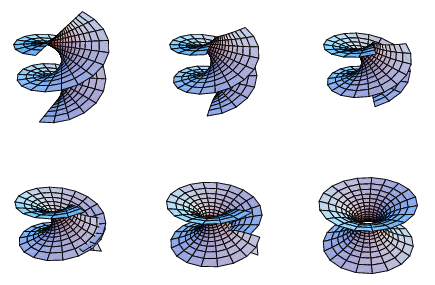
\includegraphics[width=0.5\textwidth]{HelicoidCatenoid}
\end{figure}

\begin{dem}[Teorema 22]\mbox{}
\begin{itemize}
	\item[$(\Rightarrow)$] Sea $p \in M$. Por hipótesis, $M$ y $N$ son localmente isométricas. Entonces existen $U' \subseteq M$ abierto y $V' \subseteq N$ abierto con $p \in U'$ y la isometría $f : U' \to V'$. Sea $(U,x)$ una superficie simple de $M$ en $p$ tal que $\X(U) \subseteq U'$. Consideremos $\Y : U \to \R^3$ dada por $\Y = f \circ \X$. Veamos que $\Y$ es superficie simple en $N$, ya que:
	\begin{enumerate}
	\item $\Y$ es inyectiva y diferenciable, por ser composición de funciones inyectivas y diferenciables.
	\item $\Y_1 \times \Y_2 \neq 0$.
\end{enumerate}

Tenemos que $\X$ s una superficie simple en $M$, por tanto, $\X_1 \times \X_2 \neq 0$, o equivalentemente $\{\X_1,\X_2\}$ es base de $T_q(M)$ para todo $q \in \X(U)$. Dado $q = \X(u¹_0,u²_0)$, podemos considerar la curva paramétrica $α(u²)=\X(u¹_0,u²)$, que verifica que $α(u²_0) = q$ y $α'(u²_0)=\X_1(u¹_0,u²_0)$. Además $f_{*q}α'(u²_0)=(f \circ α)'(u²_0)$. Ya que $(f\circ α)(u²)=(f \circ \X)(u¹_0,u²)=\Y(u¹_0,u²)$, tenemos que $(f\circ α)'(u²_0) = \Y_1(u²_0)$. Luego $f_{*q} \X_1(u¹_0,u²_0) = \Y_1(u¹_0,u²_0)$. Análogamente, tenemos $f_{*q} \X_2(u¹_0,u²_0)=\Y_2(u¹_0,u²_0)$.

Como $f$ es regular, $f_{*q}$ es isomorfismo. Como consecuencia, tenemos que $\{\Y_1,\Y_2\}$ son linealmente independientes o, equivalentemente, $\Y_1 \times \Y_2 \neq 0$. Luego $\Y$ es superficie simple.

Dado $(u¹_0,u²_0) \in U$, consideramos $q = \X(u¹_0,u²_0)$. Ya que $f_{*q}$ es isometría:
\begin{align*}
	g_{ij}(u¹_0,u²_0) & = I_q(\X_i(u¹_0,u²_0),\X_j(u¹_0,u²_0)) = I_{f(q)}(f_{*q}\X_i(u¹_0,u²_0),f_{*q}\X_j(u¹_0,u²_0)) \\
	& = I_{f(q)}(\Y_i(u¹_0,u²_0),\Y_j(u¹_0,u²_0)) = h_{ij}(u¹_0,u²_0)
\end{align*}

\item[$(\Rightarrow)$] Sea $p \in M$. Por hipótesis, existen $U \subseteq \R^2$ abierto y unas superficies simples $(U,\X)$ y $(U,\Y)$ tales que $p \in \X(U)$ y $g_{ij}(u¹,u²)=h_{ij}(u¹,u²)$ $\forall (u¹,u²)\in U$. Sean $U' = \X(U)  \subseteq M$ abierto y $V' = \Y(U) \subseteq N$ aberto. Sea $f : U' \to V'$ dada por $f = \Y \circ \X^{-1}$. Veamos que $f$ es isometría:
\begin{enumerate}
	\item $f$ es biyectiva y continua, por ser composición de funciones biyectivas y continuas.
	\item $f$ es regular, es decir, $f$ es diferenciable y $J_{q'} = J_{\X^{-1}(q)}$ es regular para todo $q \in U$. Si consideamos las superficie simples $(U,\X)$ y $(U,\Y)$ tenemos que:
	\[ \Y^{-1} \circ f \circ \X = \Y^{-1} \circ \Y \circ \X^{-1} \circ \X = id_U,\text{ que es }C^{∞} \]
	y $J_{q'}(\Y^{-1} \circ f \circ \X) = \begin{pmatrix}1 & 0\\0 & 1\end{pmatrix}$, que es regular.
	
	\item $f_{*q}$ es isometría $\forall q \in U'$, es decir; $f_{*q}$ conserva los módulos. Sea $q \in U'$, $q = \X(u¹_0,u²_0)$. Sea $v \in T_q(M)$, donde $v = λ¹\X_1(u¹_0,u²_0)+λ²\X_2(u¹_0,u²_0)$, con $λ¹,λ²\in\R$.
	\[ ||v||²=I_p(v,v)=(λ¹)^2 g_{11}(u_0)+(λ²)^2 g_{22}(u_0)+2λ¹λ² g_{12}(u_0) \]
	Por otro lado, $f_{*q}v = μ¹ \Y_1(u_0)+μ^2 \Y_2(u_0)$, con $μ = J_{q'} λ$. Como $J_{q'}$ es la matriz identidad, $μ=λ$.
	Por lo tanto:
	\[ ||f_{*q}||^2 = I_{f(q)}(f_{*q} v,f_{*q} v) = (μ_1)^2 h_{11}(u_0) + (μ²)^2 h_{22}(u_0) + 2 μ¹μ² h_{12}(u_0) = ||v||^2 \]
	Luego $f : U' \to V'$ es isometría. Como consecuencia, $M$ es localmente isométrica a $N$. Análogamente $N$ es localmente isométrica a $M$.
	\end{enumerate}
\end{itemize}
\end{dem}

\begin{dem}[El cilindro es estricto localmente isométrico al plano]
Sea $\X : U \to M$, donde $U=(0,a) \times (0,2\pi)$, dado por $\X(u,θ) = (r\cos θ, r \sin θu)$ una parametrización de un ciclindro $M$ de radio $r$ y eje $OZ$. Sea $p \in M$. Consideramos las superficies simples $(U,\X)$ y $(U,\Y)$ de $M$ y $N = \R^2$ tales que $p \in \X(U)$ y $g_{ij}(u,θ)=h_{ij}(u,θ)$ $\forall (u,θ) \in U$. Para ello, tomaremos $\Y(u,θ) = (rθ,0,u)$ (está elección quedará explicada en breve). Queda como ejercicio comprobar que $(U,\X)$ y $(U,\Y)$ son superficie simples.
Para $(U,\X)$:
\[ g_{11} = 1, \quad g_{12} = 0 \quad g_{22}=r^2 \]
Par $(U,\Y)$.
\[ h_{11} = 1, \quad h_{12} = 0 \quad h_{22}=r^2 \]
Por tanto, el clindro y el plano son localmente isométricos pero no isométricos.
\end{dem}
\end{document}
